\section{EXAMINATION OF THE CONSOLIDATED-UNDRAINED TEST 固结不排水试验试验}

\begin{paracol}{2}
    
    One widely used technique to estimate the undrained shear strength $S_u$ of an element of clay in the ground is to isotropically consolidate the specimen in the laboratory to a pressure equal to the effective vertical pressure in the ground, and then test the soil in undrained shear. This process involves first a reduction of effective stress and then a reapplication prior to undrained shear. For a normally consolidated specimen, for example, the stresses are reduced from the $K_0$ effective stresses to the isotropic effective stress $\overline{\sigma}_r$, and then reconsolidated isotropically to a stress equal to $\overline{\sigma}_{v0}$. During this large reduction and subsequent increase in effective stresses, and also because of the change from a $K_0$$K_0$ to an isotropic stress system, a significant volume reduction normally occurs. Many (but not all, such as \citet{Taylor1948}, p.397) soil engineers feel that this volume decrease results in an undrained shear strength which is too large. For example, see \citet{Rutledge19441155}, p.1216, \citet{Hansen1948189}, p.204, \citet{Osterberg1956}, p.70, and \citet{Bishop1960437}, p.449.

    \switchcolumn

    估算地面中黏土元素的不排水抗剪强度$S_u$的一种广泛使用的技术是在实验室中将试样各向同性地固结到等于地面中有效垂直压力的压力,然后对其进行不排水的剪切试验。该过程首先涉及减小有效应力,然后在不排水剪切之前重新施加应力。 例如,对于正常固结的试样,应力从$K_0$有效应力减小到各向同性有效应力$\overline{\sigma}_r$,然后各向同性地再固结到等于$\overline{\sigma}_{v0}$的应力。 在这种较大的减小和随后的有效应力增加期间,并且还由于从$K_0$变为各向同性应力系统,通常会发生明显的体积减小。 许多岩土工程师(但不是全部,例如\citet{Taylor1948}第397页)认为,这种体积减小会导致不排水的剪切强度过大。 例如,请参见\citet{Rutledge19441155}第1216页,\citet{Hansen1948189}第204页,\citet{Osterberg1956}第70页以及\citet{Bishop1960437}第449页。

\end{paracol}

\Paragraph{Published Methods of Correcting CIU Test Results: 修正CIU试验结果的已有方法:}

\begin{paracol}{2}
    
    Several methods have been suggested for evaluating the effects of volume change on undrained strength. These methods generally extrapolate, in various ways, a plot of $\log{}S_u$ from CIU triaxial tests versus void ratio $e$ to a value of $S_u$ corresponding to the in-situ void ratio. For example, \citet{Schmertmann1956940} draws a line through the point of intersection of lines of $\log{}S_u-e$ for CIU tests on undisturbed and remolded specimens and parallel to the estimated slope of the in situ consolidation curve. The intersection of this line with the in-situ void ratio yields the field undisturbed strength. \citet{Calhoon1956925} shifts the plot of log s versus e from CIU triaxial tests upward in proportion to the per cent disturbance of the triaxial specimens. The percent disturbance is deduced from the location of the $\log{}S_u-e$ curve from the triaxial tests in relationship to $\log{}S_u-e$ plots from oedometer tests on varying size specimens and on a remolded specimen.\footnote{
        This method assumes that only trimming produces sample disturbance, which can be very incorrect, and it neglects the effect of K on the location of c curves. 该方法假定仅对样品的修剪会产生样本干扰,这可能是非常不正确的,并且忽略了K对$\overline{\sigma}_c$曲线位置的影响。} 
    One of the simplest methods, that of \citet{Casagrande1947}, as quoted by \citet{Hvorslev1949}, suggests an extrapolation of the $\log{}S_u-e$ line from CIU tests back to the in situ void ratio as an approximate approach for obtaining $S_u$ corresponding to no volume change.

    \switchcolumn

    已经提出了几种方法来评估体积变化对不排水强度的影响。 这些方法通常以各种方式将来自CIU三轴试验的$\log{}S_u$与孔隙率$e$的关系图推导出对应于原位孔隙率的$S_u$值。 例如,\citet{Schmertmann1956940}在原状和重塑试样上进行CIU试验时,通过$\log{}S_u-e$曲线的交点画一条线,该线平行于原位固结曲线的估计斜率。 这条线与原位空隙率的交点产生了不受干扰的场强。\footnote{Need to change}\citet{Calhoon1956925}将CIU三轴试验的$\log{}S_u-e$的曲线与三轴试样的扰动百分比成比例地向上移动。 干扰百分比从三轴试验中的$\log{}S_u-e$曲线和不同尺寸的样品和重塑的样品上的固结试验得到的$\log{}S_u-e$图的位置关系中得出。\footnote{Need to change} 最简单的方法之一,如\citet{Hvorslev1949}所引用的\citet{Casagrande1947}的方法,建议将CIU试验的$\log{}S_u-e$曲线外推到原位空隙率作为获得对应于无体积变化的$S_u$的近似方法。

    \switchcolumn*

    The application of these methods to the strength data on Kawasaki Clay I, \autoref{figure:10}, yielded the values of $S_u$ corrected for volume change,\footnote{
        There are insufficient data on the other cases in \autoref{table:2} to allow similar analyses. \cntableref{table:2}中其他案例的数据不足,无法进行类似的分析。
    } shown in \autoref{table:3}. There is a wide divergence in the resulting strengths. Two of the methods yielded strengths which are too low since they are equal to, or smaller than, the 0.5 $\rm{kg/cm^2}$ from the UU tests. On the other hand, the $S_u$ from the Calhoon method is too high since CIU tests with $\overline{\sigma}_c=\overline{\sigma}_{v0}$ yielded an $S_u$ of only about 0.8 $\rm{kg/cm^2}$ (\autoref{figure:8}). Even if the Kawasaki Clay I represents an unusual case, these methods would appear to be questionable.

    \switchcolumn

    将这些方法应用于\cnfigureref{figure:10}所示的Kawasaki黏土I的强度数据后,得出的$S_u$值已针对体积变化进行了修正,如\cntableref{table:3}所示。在结果上存在很大差异。 两种方法得出的强度太低,因为它们等于或小于UU试验中的0.5$\rm{kg/cm^2}$。 另一方面,来自Calhoon方法的$S_u$太大,因为$\overline{\sigma}_c=\overline{\sigma}_{v0}$时的CIU试验得出的$S_u$仅为0.8$\rm{kg/cm^2}$(\cnfigureref{figure:8})。即使Kawasaki黏土I代表一个不寻常的情况,这些方法似乎仍然值得怀疑。

\end{paracol}

\begin{table}[!htb]
    \centering
    \caption{PREDICTION OF UNDRAINED STRENGTH AT IN SITU VOID RATIO FROM CIU TRIAXIAL TESTS BY PREVIOUS METHODS FOR KAWASAKI CLAY I.}
    \addtocounter{table}{-1}
    \vspace{-8pt}
    \renewcommand{\tablename}{表}
    \caption{川崎黏土I的先前方法从CIU三轴试验预测原位空隙率的不排水强度。}
    \vspace{4pt}
    \renewcommand{\tablename}{Table}
    \begin{threeparttable}[b]
        \begin{tabularx}{\textwidth}{ll}
            \toprule
            Method & $S_u{\rm (kg/cm^2)~for}~ \Delta{}e/(1+e_0)=0$\\
            \midrule
            \citet{Schmertmann1956940} & ~~0.3 to 0.45 \\
            \citet{Calhoon1956925} & $\sim$0.85 \\
            \citet{Casagrande1947} & $\sim$0.5 \\
            Average of unconfined\tnote{a} compression tests & ~~0.45\tnote{b} \\
            Average of $\overline{UU}$ and top one third of unconfined compression tests & ~~0.5\tnote{b} \\
            \bottomrule
        \end{tabularx}%
        \begin{tablenotes}
            \item[a] Many of the specimens contained lenses of sand, silt, or shells which caused very low unconfined strengths. 许多标本包含沙粒,粉尘或贝壳状的透镜,这些透镜的强度很低。
            \item[b] Corrected to correspond to $t_f=5$ hr. 校正为对应于 $t_f=5$小时。
        \end{tablenotes}
    \end{threeparttable}
    \label{table:3}%
\end{table}


\Paragraph{Proposed Methods of Correcting CIU Test Results: 修正CIU试验结果的建议方法:}

\begin{paracol}{2}

    One way to account for the effects on $S_u$ of the volume change upon reconsolidation is to use the Hvorslev \citet{Hvorslev1960169}, p. 210 or \citet{Bishop1962}, p. 166 which can be expressed as follows: $\big(\dfrac{1}{2}(\sigma_1-\sigma_3)_f$ is replaced by $S_u$ since only undrained shear strength is considered$\big)$

    \switchcolumn

    解决固结对体积变化$S_u$的影响的一种方法是使用Hvorslev参数\citet{Hvorslev1960169}第210页或\citet{Bishop1962}第166页,可以表示为:$\big(\dfrac{1}{2}(\sigma_1-\sigma_3)_f$被$S_u$代替,因为只考虑了不排水的剪切强度$\big)$

\end{paracol}

\begin{align}
    S_u=H\overline{\sigma}_e+\overline{\sigma}_{3f}\tan\overline{\theta}_e
    \label{equation:2}
\end{align}

\begin{paracol}{2}

    \noindent{}where:\\
    \newlength\length
    \settowidth{\length}{$\tan\overline{\theta}_e$}
    \makebox[\length][l]{H} = $K(\cos\overline{\phi}_e)/(1-\sin\overline{\phi}_e)$, \\
    \makebox[\length][l]{$\tan\overline{\theta}_e$} = $(\sin\overline{\phi}_e)/(1-\sin\overline{\phi}_e)$, \\
    \makebox[\length][l]{K} = $\overline{c}_e/\overline{\sigma}_e$, \\
    \makebox[\length][l]{$\overline{c}_e$} = Hvorslev cohesion, \\
    \makebox[\length][l]{$\overline{\phi}_e$} = Hvorslev friction angle, and \\
    \makebox[\length][l]{$\overline{\sigma}_e$} = Hvorslev equivalent consolidation pressure. 

    \switchcolumn

    \noindent{}式中:\\
    \makebox[\length][l]{H} = $K(\cos\overline{\phi}_e)/(1-\sin\overline{\phi}_e)$, \\
    \makebox[\length][l]{$\tan\overline{\theta}_e$} = $(\sin\overline{\phi}_e)/(1-\sin\overline{\phi}_e)$,\\
    \makebox[\length][l]{K} = $\overline{c}_e/\overline{\sigma}_e$, \\
    \makebox[\length][l]{$\overline{c}_e$} = Hvorslev粘聚力, \\
    \makebox[\length][l]{$\overline{\phi}_e$} = Hvorslev摩擦角,以及 \\
    \makebox[\length][l]{$\overline{\sigma}_e$} = Hvorslev等效固结压力。

    \switchcolumn*

    \noindent{}If two specimens were consolidated to the same pressure, but had different water contents and hence different values of $\overline{\sigma}_e$, then the difference in $S_u$ for undrained shear could be reflected in changes in both $H\overline{\sigma}_e$ and $\overline{\sigma}_{3f}\tan\overline{\theta}_e$. However, if $\overline{\sigma}_{3f}$ were independent of the water content change, the difference in $S_u$ could be calculated from the change in $H\overline{\sigma}_e$, assuming of course, that H and $H\overline{\theta}_e$ were constants for the soil.\footnote{
        \citet{Bjerrum1960101} show that H varies with consolidation pressure for undisturbed specimens of Lilla Edet clay, which is believed to have a significant amount of natural eementation. \citet{Bjerrum1960101}表明,对于Lilla Edet黏土的未扰动标本,H随固结压力的变化而变化,该黏土被认为具有大量的自然胶结作用。
    }

    \switchcolumn

    \noindent{}如果将两个试样固结到相同的压力下,但是含水量不同,因此$\overline{\sigma}_e$值也不同,则不排水剪切的$S_u$差异可以反映在$H\overline{\sigma}_e$和$\overline{\sigma}_{3f}\tan\overline{\theta}_e$的变化中。但是,如果$\overline{\sigma}_{3f}$与含水量的变化无关,则可以根据$H\overline{\sigma}_e$的变化来计算$S_u$的差,当然,假设H和$H\overline{\theta}_e$是土体的常数。

\end{paracol}
    
\begin{figure}[!htbp]
    \centering
    \begin{minipage}[t]{0.48\textwidth}
        \centering
        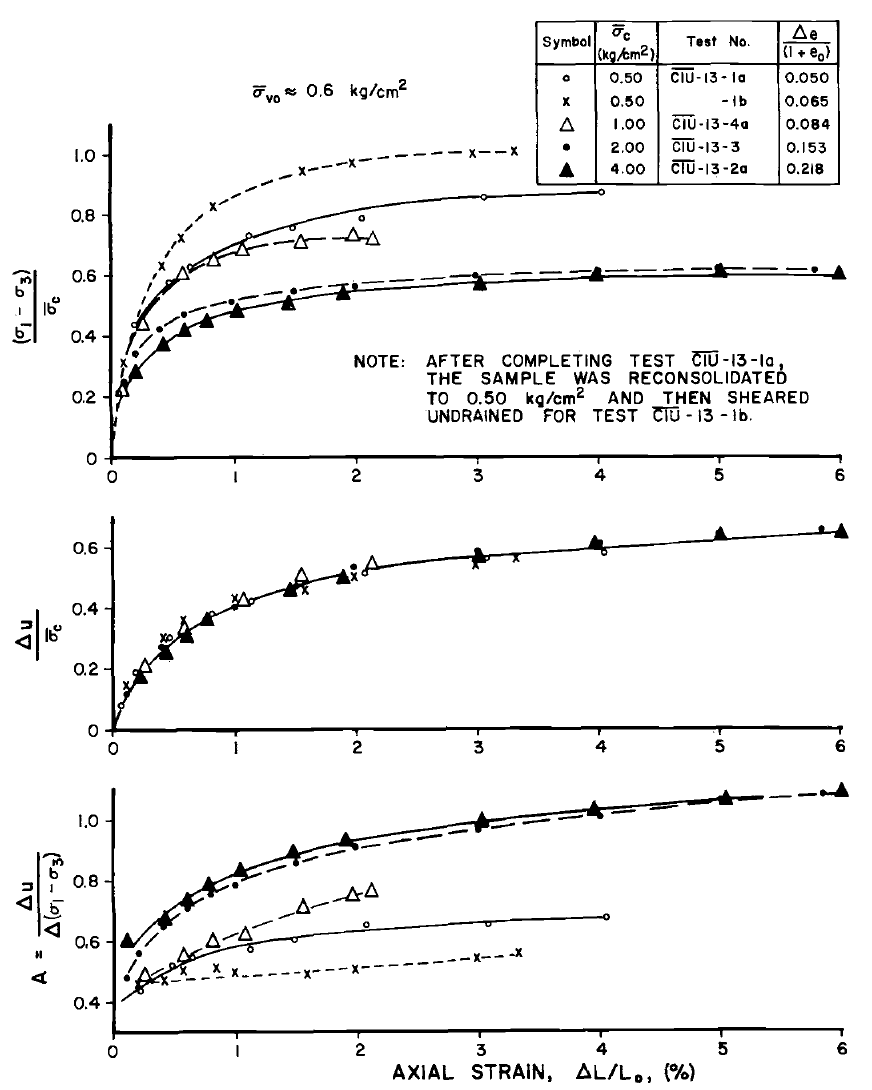
\includegraphics[width=0.9\textwidth]{figures/figure-13.png}
        \caption{Effect of Consolidation Pressure and Reconsolidation on the Stress-Strain Behavior of Lagunillas Clay.}
        \vspace{-5pt}
        \addtocounter{figure}{-1}
        \renewcommand{\figurename}{图}
        \caption{固结压力和再固结对Lagunillas黏土应力应变行为的影响。}
        \label{figure:13}
        \renewcommand{\figurename}{Figure}
    \end{minipage}
    \begin{minipage}[t]{0.48\textwidth}
        \centering
        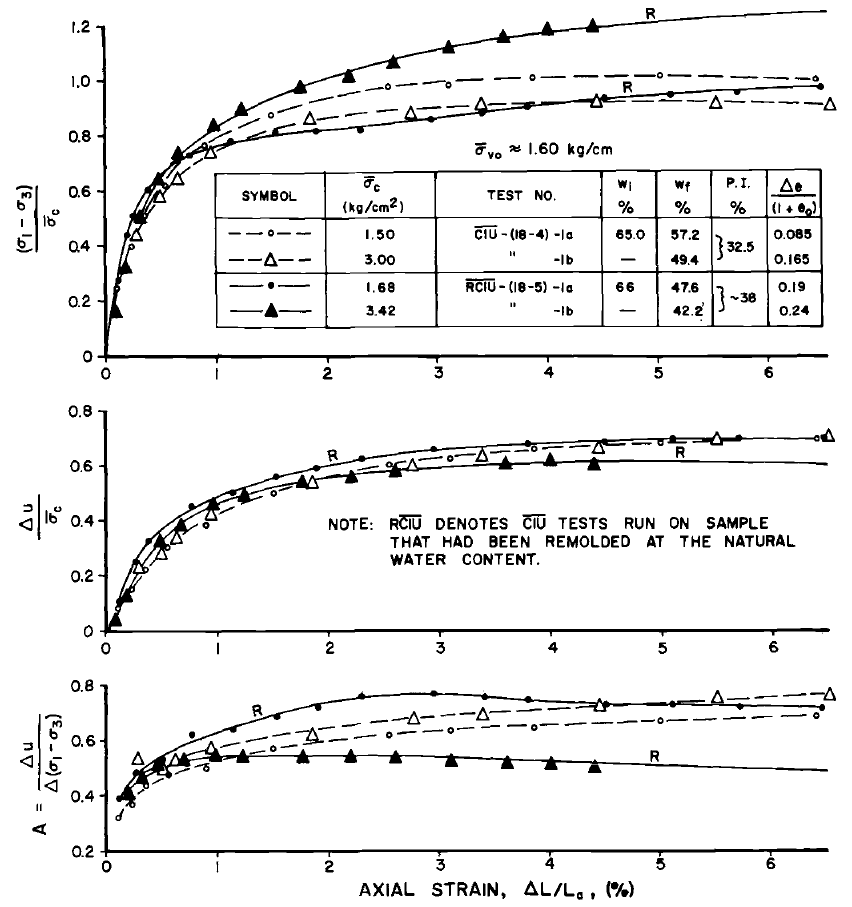
\includegraphics[width=0.9\textwidth]{figures/figure-14.png}
        \caption{Effect of Consolidation Pressure and Remolding on the Stress-Strain Behavior of Kawasaki Clay I.}
        \vspace{-5pt}
        \addtocounter{figure}{-1}
        \renewcommand{\figurename}{图}
        \caption{固结压力和重塑对Kawasaki黏土I应力-应变行为的影响。}
        \label{figure:14}
        \renewcommand{\figurename}{Figure}
    \end{minipage}
\end{figure}

\begin{paracol}{2}

    Since $\overline{\sigma}_{3f}$ is directly related to the excess pore pressure at failure, one can look at the effects of volume change on the pore pressure behavior of $\overline{CIU}$ tests. Such data for the Lagunillas clay and the Kawasaki Clay I are presented in \autoref{figure:13} and \autoref{figure:14}. The data show that $\Delta{}u/\overline{\sigma}_c$ versus strain is practically independent of (1) consolidation pressure for $\overline{\sigma}_c$ values greater than $\overline{\sigma}_{ps}$, even though the value of volumetric strain compared to the in situ value varies considerably with consolidation pressure (\autoref{figure:9} and \autoref{figure:10}), (2) reconsolidation, with resultant volume decrease, after undrained shear (Test $\overline{CIU}-13-1(b)$ in \autoref{figure:13}), and (3) remolding at the natural water content with subsequent consolidation and very large volume changes (Tests $R\overline{CIU}-(18-5)-1(a)$ and $-1(b)$ in \autoref{figure:14}). As a reasonable approximation it is therefore assumed that the volume change caused by the consolidation of $\overline{CIU}$ specimens to pressures between $\overline{\sigma}_{ps}$ and $\overline{\sigma}_{v0}$ has little effect on $\Delta{}u/\overline{\sigma}_c$ during undrained shear, and that the strain at failure is also unaltered. The decrease in $S_u$ is then calculated from the change in Hvorslev cohesion, $H\Delta{}\overline{\sigma}_e$, commensurate with the decrease in volume from the in situ condition, $\Delta{}e/(1+e_0)$. An example is given in the next section.

    \switchcolumn

    由于$\overline{\sigma}_{3f}$与失效时多余的孔隙压力直接相关,因此可以查看体积变化对$\overline{CIU}$试验的孔隙压力行为的影响。Lagunillas黏土和Kawasaki黏土I的这些数据在\cnfigureref{figure:13}和\cnfigureref{figure:14}显示。数据显示$\Delta{}u/\overline{\sigma}_c$与应变的关系实际上与(1)超过$\overline{\sigma}_{ps}$的$\overline{\sigma}_c$值的固结压力,即使体积应变的值与原位试验值相比随固结压力变化很大(\cnfigureref{figure:9}和\cnfigureref{figure:10}),(2)在不排水的剪切之后重新固结,导致体积减小(\cnfigureref{figure:13}中的试验$\overline{CIU}-13-1(b)$)以及(3)在天然含水量下重塑并随后固结以及非常大的体积变化(\cnfigureref{figure:14}中的$R\overline{CIU}-(18-5)-1(a)$和$-1(b)$试验)无关。因此,作为合理的近似值,可以假设在不排水的剪切过程中,在固结应力为$\overline{\sigma}_{ps}$和$\overline{\sigma}_{v0}$之间时,由$\overline{CIU}$试样的固结引起的体积变化对$\Delta{}u/\overline{\sigma}_c$的影响很小,并且破坏时的应变也没有改变。$S_u$的减少可通过Hvorslev内聚力$H\Delta{}\overline{\sigma}_e$的变化与原位条件下体积的减少$\Delta{}e/(1+e_0)$相称来计算。下一节将给出一个示例。

    \switchcolumn*

    Another possible approach to the problem of assessing the effects of volume change would be to use the results of CU tests at consolidation pressures much larger than $\overline{\sigma}_{v0}$, where the effects of specimen disturbance might be minimized \citet{Marsal1957229}, p. 194, \citet{Casagrande1953}, p. 33. This method, as with previous ones, requires negligible changes in soil structure with consolidation pressure. If the value of $S_u$ corresponding to perfect sampling is desired, CA-UU tests should be used with consolidation pressures at least two to four times $\overline{\sigma}_{v0}$.

    \switchcolumn

    评估体积变化影响的另一种可能的方法是,在固结压力远大于$\overline{\sigma}_{v0}$的情况下使用CU试验的结果,在这种情况下,样品扰动的影响可能会最小化\citet{Marsal1957229}第194页,\citet{Casagrande1953}第33页。与以前一样,这种方法要求土壤结构随固结压力的变化可忽略不计。 如果需要与完美采样相对应的$S_u$值,则应使用固结压力至少为$\overline{\sigma}_{v0}$的2-4倍的CA-UU试验。

\end{paracol}